% Options for packages loaded elsewhere
\PassOptionsToPackage{unicode}{hyperref}
\PassOptionsToPackage{hyphens}{url}
%
\documentclass[
]{book}
\usepackage{amsmath,amssymb}
\usepackage{iftex}
\ifPDFTeX
  \usepackage[T1]{fontenc}
  \usepackage[utf8]{inputenc}
  \usepackage{textcomp} % provide euro and other symbols
\else % if luatex or xetex
  \usepackage{unicode-math} % this also loads fontspec
  \defaultfontfeatures{Scale=MatchLowercase}
  \defaultfontfeatures[\rmfamily]{Ligatures=TeX,Scale=1}
\fi
\usepackage{lmodern}
\ifPDFTeX\else
  % xetex/luatex font selection
\fi
% Use upquote if available, for straight quotes in verbatim environments
\IfFileExists{upquote.sty}{\usepackage{upquote}}{}
\IfFileExists{microtype.sty}{% use microtype if available
  \usepackage[]{microtype}
  \UseMicrotypeSet[protrusion]{basicmath} % disable protrusion for tt fonts
}{}
\makeatletter
\@ifundefined{KOMAClassName}{% if non-KOMA class
  \IfFileExists{parskip.sty}{%
    \usepackage{parskip}
  }{% else
    \setlength{\parindent}{0pt}
    \setlength{\parskip}{6pt plus 2pt minus 1pt}}
}{% if KOMA class
  \KOMAoptions{parskip=half}}
\makeatother
\usepackage{xcolor}
\usepackage{color}
\usepackage{fancyvrb}
\newcommand{\VerbBar}{|}
\newcommand{\VERB}{\Verb[commandchars=\\\{\}]}
\DefineVerbatimEnvironment{Highlighting}{Verbatim}{commandchars=\\\{\}}
% Add ',fontsize=\small' for more characters per line
\usepackage{framed}
\definecolor{shadecolor}{RGB}{248,248,248}
\newenvironment{Shaded}{\begin{snugshade}}{\end{snugshade}}
\newcommand{\AlertTok}[1]{\textcolor[rgb]{0.94,0.16,0.16}{#1}}
\newcommand{\AnnotationTok}[1]{\textcolor[rgb]{0.56,0.35,0.01}{\textbf{\textit{#1}}}}
\newcommand{\AttributeTok}[1]{\textcolor[rgb]{0.13,0.29,0.53}{#1}}
\newcommand{\BaseNTok}[1]{\textcolor[rgb]{0.00,0.00,0.81}{#1}}
\newcommand{\BuiltInTok}[1]{#1}
\newcommand{\CharTok}[1]{\textcolor[rgb]{0.31,0.60,0.02}{#1}}
\newcommand{\CommentTok}[1]{\textcolor[rgb]{0.56,0.35,0.01}{\textit{#1}}}
\newcommand{\CommentVarTok}[1]{\textcolor[rgb]{0.56,0.35,0.01}{\textbf{\textit{#1}}}}
\newcommand{\ConstantTok}[1]{\textcolor[rgb]{0.56,0.35,0.01}{#1}}
\newcommand{\ControlFlowTok}[1]{\textcolor[rgb]{0.13,0.29,0.53}{\textbf{#1}}}
\newcommand{\DataTypeTok}[1]{\textcolor[rgb]{0.13,0.29,0.53}{#1}}
\newcommand{\DecValTok}[1]{\textcolor[rgb]{0.00,0.00,0.81}{#1}}
\newcommand{\DocumentationTok}[1]{\textcolor[rgb]{0.56,0.35,0.01}{\textbf{\textit{#1}}}}
\newcommand{\ErrorTok}[1]{\textcolor[rgb]{0.64,0.00,0.00}{\textbf{#1}}}
\newcommand{\ExtensionTok}[1]{#1}
\newcommand{\FloatTok}[1]{\textcolor[rgb]{0.00,0.00,0.81}{#1}}
\newcommand{\FunctionTok}[1]{\textcolor[rgb]{0.13,0.29,0.53}{\textbf{#1}}}
\newcommand{\ImportTok}[1]{#1}
\newcommand{\InformationTok}[1]{\textcolor[rgb]{0.56,0.35,0.01}{\textbf{\textit{#1}}}}
\newcommand{\KeywordTok}[1]{\textcolor[rgb]{0.13,0.29,0.53}{\textbf{#1}}}
\newcommand{\NormalTok}[1]{#1}
\newcommand{\OperatorTok}[1]{\textcolor[rgb]{0.81,0.36,0.00}{\textbf{#1}}}
\newcommand{\OtherTok}[1]{\textcolor[rgb]{0.56,0.35,0.01}{#1}}
\newcommand{\PreprocessorTok}[1]{\textcolor[rgb]{0.56,0.35,0.01}{\textit{#1}}}
\newcommand{\RegionMarkerTok}[1]{#1}
\newcommand{\SpecialCharTok}[1]{\textcolor[rgb]{0.81,0.36,0.00}{\textbf{#1}}}
\newcommand{\SpecialStringTok}[1]{\textcolor[rgb]{0.31,0.60,0.02}{#1}}
\newcommand{\StringTok}[1]{\textcolor[rgb]{0.31,0.60,0.02}{#1}}
\newcommand{\VariableTok}[1]{\textcolor[rgb]{0.00,0.00,0.00}{#1}}
\newcommand{\VerbatimStringTok}[1]{\textcolor[rgb]{0.31,0.60,0.02}{#1}}
\newcommand{\WarningTok}[1]{\textcolor[rgb]{0.56,0.35,0.01}{\textbf{\textit{#1}}}}
\usepackage{longtable,booktabs,array}
\usepackage{calc} % for calculating minipage widths
% Correct order of tables after \paragraph or \subparagraph
\usepackage{etoolbox}
\makeatletter
\patchcmd\longtable{\par}{\if@noskipsec\mbox{}\fi\par}{}{}
\makeatother
% Allow footnotes in longtable head/foot
\IfFileExists{footnotehyper.sty}{\usepackage{footnotehyper}}{\usepackage{footnote}}
\makesavenoteenv{longtable}
\usepackage{graphicx}
\makeatletter
\def\maxwidth{\ifdim\Gin@nat@width>\linewidth\linewidth\else\Gin@nat@width\fi}
\def\maxheight{\ifdim\Gin@nat@height>\textheight\textheight\else\Gin@nat@height\fi}
\makeatother
% Scale images if necessary, so that they will not overflow the page
% margins by default, and it is still possible to overwrite the defaults
% using explicit options in \includegraphics[width, height, ...]{}
\setkeys{Gin}{width=\maxwidth,height=\maxheight,keepaspectratio}
% Set default figure placement to htbp
\makeatletter
\def\fps@figure{htbp}
\makeatother
\setlength{\emergencystretch}{3em} % prevent overfull lines
\providecommand{\tightlist}{%
  \setlength{\itemsep}{0pt}\setlength{\parskip}{0pt}}
\setcounter{secnumdepth}{5}
\ifLuaTeX
  \usepackage{selnolig}  % disable illegal ligatures
\fi
\usepackage[]{natbib}
\bibliographystyle{apalike}
\nocite{*}
\IfFileExists{bookmark.sty}{\usepackage{bookmark}}{\usepackage{hyperref}}
\IfFileExists{xurl.sty}{\usepackage{xurl}}{} % add URL line breaks if available
\urlstyle{same}
\hypersetup{
  pdftitle={Supplemental Material for `Optimizing Model Performance and Fairness Through Evolved Sample Weights'},
  pdfauthor={Anil Kumar Saini, Jose Guadalupe Hernandez, Emily F. Wong, Jason H. Moore},
  hidelinks,
  pdfcreator={LaTeX via pandoc}}

\title{Supplemental Material for `Optimizing Model Performance and Fairness Through Evolved Sample Weights'}
\author{Anil Kumar Saini, Jose Guadalupe Hernandez, Emily F. Wong, Jason H. Moore}
\date{2024-07-31}

\begin{document}
\maketitle

{
\setcounter{tocdepth}{1}
\tableofcontents
}
\hypertarget{introduction}{%
\chapter{Introduction}\label{introduction}}

This is not intended as a stand-alone document, but as a companion to our manuscript.

\hypertarget{contributing-authors}{%
\section{Contributing authors}\label{contributing-authors}}

\begin{itemize}
\tightlist
\item
  \href{https://theaksaini.github.io/}{Anil Kumar Saini}
\item
  \href{https://jgh9094.github.io/}{Jose Guadalupe Hernandez}
\item
  \href{https://www.cedars-sinai.edu/research-education/research/labs/bright/members.html}{Emily F. Wong}
\item
  \href{https://jasonhmoore.org/}{Jason H. Moore}
\end{itemize}

\hypertarget{about-our-supplemental-material}{%
\section{About our supplemental material}\label{about-our-supplemental-material}}

As you may have noticed (unless you're reading a pdf version of this), our supplemental material is hosted using \href{https://pages.github.com/}{GitHub pages}.
We compiled our data analyses and supplemental documentation into this nifty web-accessible book using \href{https://bookdown.org}{bookdown}.

The code used for this supplemental material can be found in \href{https://github.com/jgh9094/GPTP-2024-Lexicase-Analysis}{this GitHub repository}.

Our supplemental material includes the following:

\begin{itemize}
\tightlist
\item
  Heart disease results (Section \ref{heart-disease})
\item
  Student math results (Section \ref{student-math})
\item
  Student por results (Section \ref{student-por})
\item
  CreditG results (Section \ref{creditg})
\item
  Titanic results (Section \ref{titanic})
\item
  US Crime results (Section \ref{us-crime})
\item
  Compas Violent results (Section \ref{compas-violent})
\item
  NLSY results (Section \ref{nlsy})
\item
  Compas results (Section \ref{compas})
\item
  Speed dating results (Section \ref{speeddating})
\item
  PMAD EPDS results (Section \ref{pmad-epds})
\item
  PMAD PHQ results (Section \ref{pmad-phq})
\end{itemize}

\hypertarget{supplemental-material-setup}{%
\section{Supplemental material setup}\label{supplemental-material-setup}}

\hypertarget{required-packages-and-variables}{%
\subsection{Required packages and variables}\label{required-packages-and-variables}}

Variable set up.

\begin{Shaded}
\begin{Highlighting}[]
\FunctionTok{library}\NormalTok{(ggplot2)}
\FunctionTok{library}\NormalTok{(cowplot)}
\FunctionTok{library}\NormalTok{(dplyr)}
\FunctionTok{library}\NormalTok{(PupillometryR)}

\NormalTok{NAMES }\OtherTok{\textless{}{-}} \FunctionTok{c}\NormalTok{(}\StringTok{\textquotesingle{}Evolved\textquotesingle{}}\NormalTok{,}\StringTok{\textquotesingle{}Calculated\textquotesingle{}}\NormalTok{,}\StringTok{\textquotesingle{}None\textquotesingle{}}\NormalTok{)}
\NormalTok{TASKS }\OtherTok{\textless{}{-}} \FunctionTok{c}\NormalTok{(}\StringTok{\textquotesingle{}heart\_disease\textquotesingle{}}\NormalTok{, }\StringTok{\textquotesingle{}student\_math\textquotesingle{}}\NormalTok{, }\StringTok{\textquotesingle{}student\_por\textquotesingle{}}\NormalTok{, }\StringTok{\textquotesingle{}creditg\textquotesingle{}}\NormalTok{, }\StringTok{\textquotesingle{}titanic\textquotesingle{}}\NormalTok{, }\StringTok{\textquotesingle{}us\_crime\textquotesingle{}}\NormalTok{, }\StringTok{\textquotesingle{}compas\_violent\textquotesingle{}}\NormalTok{, }\StringTok{\textquotesingle{}nlsy\textquotesingle{}}\NormalTok{, }\StringTok{\textquotesingle{}compas\textquotesingle{}}\NormalTok{, }\StringTok{\textquotesingle{}speeddating\textquotesingle{}}\NormalTok{,}\StringTok{\textquotesingle{}pmad\_epds\textquotesingle{}}\NormalTok{, }\StringTok{\textquotesingle{}pmad\_epds\_rus\textquotesingle{}}\NormalTok{, }\StringTok{\textquotesingle{}pmad\_phq\textquotesingle{}}\NormalTok{, }\StringTok{\textquotesingle{}pmad\_phq\_rus\textquotesingle{}}\NormalTok{)}
\NormalTok{SHAPE }\OtherTok{\textless{}{-}} \FunctionTok{c}\NormalTok{(}\DecValTok{21}\NormalTok{,}\DecValTok{24}\NormalTok{,}\DecValTok{22}\NormalTok{)}
\NormalTok{cb\_palette }\OtherTok{\textless{}{-}} \FunctionTok{c}\NormalTok{(}\StringTok{\textquotesingle{}\#D81B60\textquotesingle{}}\NormalTok{,}\StringTok{\textquotesingle{}\#1E88E5\textquotesingle{}}\NormalTok{,}\StringTok{\textquotesingle{}\#FFC107\textquotesingle{}}\NormalTok{)}
\NormalTok{TSIZE }\OtherTok{\textless{}{-}} \DecValTok{19}

\NormalTok{p\_theme }\OtherTok{\textless{}{-}} \FunctionTok{theme}\NormalTok{(}
  \AttributeTok{plot.title =} \FunctionTok{element\_text}\NormalTok{( }\AttributeTok{face =} \StringTok{"bold"}\NormalTok{, }\AttributeTok{size =} \DecValTok{22}\NormalTok{, }\AttributeTok{hjust=}\FloatTok{0.5}\NormalTok{),}
  \AttributeTok{panel.border =} \FunctionTok{element\_blank}\NormalTok{(),}
  \AttributeTok{panel.grid.minor =} \FunctionTok{element\_blank}\NormalTok{(),}
  \AttributeTok{legend.title=}\FunctionTok{element\_text}\NormalTok{(}\AttributeTok{size=}\DecValTok{18}\NormalTok{),}
  \AttributeTok{legend.text=}\FunctionTok{element\_text}\NormalTok{(}\AttributeTok{size=}\DecValTok{18}\NormalTok{),}
  \AttributeTok{axis.title =} \FunctionTok{element\_text}\NormalTok{(}\AttributeTok{size=}\DecValTok{18}\NormalTok{),}
  \AttributeTok{axis.text =} \FunctionTok{element\_text}\NormalTok{(}\AttributeTok{size=}\DecValTok{14}\NormalTok{),}
  \AttributeTok{legend.position=}\StringTok{"bottom"}\NormalTok{,}
  \AttributeTok{panel.background =} \FunctionTok{element\_rect}\NormalTok{(}\AttributeTok{fill =} \StringTok{"\#f1f2f5"}\NormalTok{,}
                                  \AttributeTok{colour =} \StringTok{"white"}\NormalTok{,}
                                  \AttributeTok{linewidth =} \FloatTok{0.5}\NormalTok{, }\AttributeTok{linetype =} \StringTok{"solid"}\NormalTok{)}
\NormalTok{)}

\NormalTok{testing }\OtherTok{\textless{}{-}} \FunctionTok{read.csv}\NormalTok{(}\FunctionTok{paste}\NormalTok{(}\StringTok{\textquotesingle{}./\textquotesingle{}}\NormalTok{, }\StringTok{\textquotesingle{}hv\_test.csv\textquotesingle{}}\NormalTok{, }\AttributeTok{sep =} \StringTok{""}\NormalTok{, }\AttributeTok{collapse =} \ConstantTok{NULL}\NormalTok{), }\AttributeTok{header =} \ConstantTok{TRUE}\NormalTok{, }\AttributeTok{stringsAsFactors =} \ConstantTok{FALSE}\NormalTok{)}
\NormalTok{testing}\SpecialCharTok{$}\NormalTok{exp }\OtherTok{\textless{}{-}} \FunctionTok{gsub}\NormalTok{(}\StringTok{\textquotesingle{}Evolved Weights\textquotesingle{}}\NormalTok{, }\StringTok{\textquotesingle{}Evolved\textquotesingle{}}\NormalTok{, testing}\SpecialCharTok{$}\NormalTok{ex)}
\NormalTok{testing}\SpecialCharTok{$}\NormalTok{exp }\OtherTok{\textless{}{-}} \FunctionTok{gsub}\NormalTok{(}\StringTok{\textquotesingle{}Calculated Weights\textquotesingle{}}\NormalTok{, }\StringTok{\textquotesingle{}Calculated\textquotesingle{}}\NormalTok{, testing}\SpecialCharTok{$}\NormalTok{ex)}
\NormalTok{testing}\SpecialCharTok{$}\NormalTok{exp }\OtherTok{\textless{}{-}} \FunctionTok{gsub}\NormalTok{(}\StringTok{\textquotesingle{}No Weights\textquotesingle{}}\NormalTok{, }\StringTok{\textquotesingle{}None\textquotesingle{}}\NormalTok{, testing}\SpecialCharTok{$}\NormalTok{ex)}
\NormalTok{testing}\SpecialCharTok{$}\NormalTok{exp }\OtherTok{\textless{}{-}} \FunctionTok{factor}\NormalTok{(testing}\SpecialCharTok{$}\NormalTok{exp, }\AttributeTok{levels =}\NormalTok{ NAMES)}
\end{Highlighting}
\end{Shaded}

\hypertarget{helper-functions}{%
\subsection{Helper functions}\label{helper-functions}}

Function to plot hypervolume results

\begin{Shaded}
\begin{Highlighting}[]
  \CommentTok{\# function to plot hyper{-}volume data}
\NormalTok{  volume\_plotter }\OtherTok{\textless{}{-}} \ControlFlowTok{function}\NormalTok{(data, id)}
\NormalTok{  \{}
    \FunctionTok{ggplot}\NormalTok{(data, }\FunctionTok{aes}\NormalTok{(}\AttributeTok{x =}\NormalTok{ exp, }\AttributeTok{y =}\NormalTok{ hv, }\AttributeTok{color =}\NormalTok{ exp, }\AttributeTok{fill =}\NormalTok{ exp, }\AttributeTok{shape =}\NormalTok{ exp)) }\SpecialCharTok{+}
    \FunctionTok{geom\_flat\_violin}\NormalTok{(}\AttributeTok{position =} \FunctionTok{position\_nudge}\NormalTok{(}\AttributeTok{x =}\NormalTok{ .}\DecValTok{1}\NormalTok{, }\AttributeTok{y =} \DecValTok{0}\NormalTok{), }\AttributeTok{scale =} \StringTok{\textquotesingle{}width\textquotesingle{}}\NormalTok{, }\AttributeTok{alpha =} \FloatTok{0.2}\NormalTok{, }\AttributeTok{width =} \FloatTok{1.5}\NormalTok{) }\SpecialCharTok{+}
    \FunctionTok{geom\_boxplot}\NormalTok{(}\AttributeTok{color =} \StringTok{\textquotesingle{}black\textquotesingle{}}\NormalTok{, }\AttributeTok{width =}\NormalTok{ .}\DecValTok{07}\NormalTok{, }\AttributeTok{outlier.shape =} \ConstantTok{NA}\NormalTok{, }\AttributeTok{alpha =} \FloatTok{0.0}\NormalTok{, }\AttributeTok{size =} \FloatTok{1.0}\NormalTok{, }\AttributeTok{position =} \FunctionTok{position\_nudge}\NormalTok{(}\AttributeTok{x =}\NormalTok{ .}\DecValTok{18}\NormalTok{, }\AttributeTok{y =} \DecValTok{0}\NormalTok{)) }\SpecialCharTok{+}
    \FunctionTok{geom\_point}\NormalTok{(}\AttributeTok{position =} \FunctionTok{position\_jitter}\NormalTok{(}\AttributeTok{width =} \FloatTok{0.02}\NormalTok{, }\AttributeTok{height =} \FloatTok{0.0001}\NormalTok{), }\AttributeTok{size =} \FloatTok{1.5}\NormalTok{, }\AttributeTok{alpha =} \FloatTok{1.0}\NormalTok{) }\SpecialCharTok{+}
    \FunctionTok{scale\_y\_continuous}\NormalTok{(}
      \AttributeTok{name=}\StringTok{"Volume"}\NormalTok{,}
\NormalTok{    ) }\SpecialCharTok{+}
    \FunctionTok{scale\_x\_discrete}\NormalTok{(}
      \AttributeTok{name=}\StringTok{"Strategy"}
\NormalTok{    )}\SpecialCharTok{+}
    \FunctionTok{scale\_shape\_manual}\NormalTok{(}\AttributeTok{values=}\NormalTok{SHAPE, }\AttributeTok{name=}\StringTok{"Weight}\SpecialCharTok{\textbackslash{}n}\StringTok{Strategy"}\NormalTok{) }\SpecialCharTok{+}
    \FunctionTok{scale\_colour\_manual}\NormalTok{(}\AttributeTok{values =}\NormalTok{ cb\_palette, }\AttributeTok{name=}\StringTok{"Weight}\SpecialCharTok{\textbackslash{}n}\StringTok{Strategy"}\NormalTok{) }\SpecialCharTok{+}
    \FunctionTok{scale\_fill\_manual}\NormalTok{(}\AttributeTok{values =}\NormalTok{ cb\_palette, }\AttributeTok{name=}\StringTok{"Weight}\SpecialCharTok{\textbackslash{}n}\StringTok{Strategy"}\NormalTok{) }\SpecialCharTok{+}
    \FunctionTok{ggtitle}\NormalTok{(TASKS[id])}\SpecialCharTok{+}
\NormalTok{    p\_theme }\SpecialCharTok{+} \FunctionTok{coord\_flip}\NormalTok{()}
\NormalTok{  \}}
\end{Highlighting}
\end{Shaded}

Function to summarize hypervolume results

\begin{Shaded}
\begin{Highlighting}[]
\CommentTok{\# function to plot hyper{-}volume data}
\NormalTok{volume\_summarize }\OtherTok{\textless{}{-}} \ControlFlowTok{function}\NormalTok{(data)}
\NormalTok{  \{}
\NormalTok{    data }\SpecialCharTok{\%\textgreater{}\%}
    \FunctionTok{group\_by}\NormalTok{(exp) }\SpecialCharTok{\%\textgreater{}\%}
\NormalTok{    dplyr}\SpecialCharTok{::}\FunctionTok{summarise}\NormalTok{(}
      \AttributeTok{count =} \FunctionTok{n}\NormalTok{(),}
      \AttributeTok{na\_cnt =} \FunctionTok{sum}\NormalTok{(}\FunctionTok{is.na}\NormalTok{(hv)),}
      \AttributeTok{min =} \FunctionTok{min}\NormalTok{(hv, }\AttributeTok{na.rm =} \ConstantTok{TRUE}\NormalTok{),}
      \AttributeTok{median =} \FunctionTok{median}\NormalTok{(hv, }\AttributeTok{na.rm =} \ConstantTok{TRUE}\NormalTok{),}
      \AttributeTok{mean =} \FunctionTok{mean}\NormalTok{(hv, }\AttributeTok{na.rm =} \ConstantTok{TRUE}\NormalTok{),}
      \AttributeTok{max =} \FunctionTok{max}\NormalTok{(hv, }\AttributeTok{na.rm =} \ConstantTok{TRUE}\NormalTok{),}
      \AttributeTok{IQR =} \FunctionTok{IQR}\NormalTok{(hv, }\AttributeTok{na.rm =} \ConstantTok{TRUE}\NormalTok{)}
\NormalTok{    )}
\NormalTok{  \}}
\end{Highlighting}
\end{Shaded}

\hypertarget{heart-disease}{%
\chapter{Heart Disease}\label{heart-disease}}

Here we report the \textbf{hypervolume} achived by evaluating the performance of each solution wihtin the Pareto front on the test set of the \texttt{heart\_disease} dataset.

\begin{Shaded}
\begin{Highlighting}[]
\CommentTok{\# heart{-}disease data}
\NormalTok{data }\OtherTok{\textless{}{-}} \FunctionTok{filter}\NormalTok{(testing, dataset }\SpecialCharTok{==} \StringTok{"heart\_disease"}\NormalTok{)}
\end{Highlighting}
\end{Shaded}

\hypertarget{hypervolume}{%
\section{Hypervolume}\label{hypervolume}}

\begin{Shaded}
\begin{Highlighting}[]
\FunctionTok{volume\_plotter}\NormalTok{(data,}\DecValTok{1}\NormalTok{)}
\end{Highlighting}
\end{Shaded}

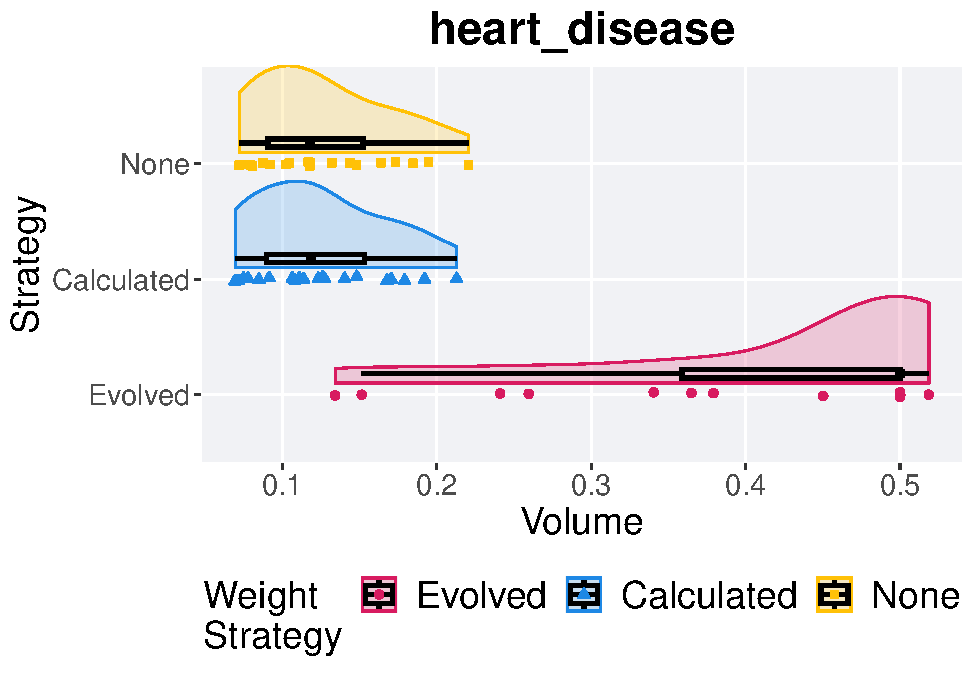
\includegraphics[width=1\linewidth]{evolved-sample-weights-supplemental_files/figure-latex/hd-hv-plt-1}

\hypertarget{summary-stats}{%
\subsection{Summary stats}\label{summary-stats}}

\begin{Shaded}
\begin{Highlighting}[]
\FunctionTok{volume\_summarize}\NormalTok{(data)}
\end{Highlighting}
\end{Shaded}

\begin{verbatim}
## # A tibble: 3 x 8
##   exp        count na_cnt    min median  mean   max    IQR
##   <fct>      <int>  <int>  <dbl>  <dbl> <dbl> <dbl>  <dbl>
## 1 Evolved       20      0 0.134   0.5   0.417 0.519 0.141 
## 2 Calculated    20      0 0.0695  0.119 0.125 0.213 0.0633
## 3 None          20      0 0.0722  0.118 0.126 0.221 0.0613
\end{verbatim}

\hypertarget{kruskal-wallis-test}{%
\subsection{Kruskal-Wallis test}\label{kruskal-wallis-test}}

Detected differences between weight strategies.

\begin{Shaded}
\begin{Highlighting}[]
\FunctionTok{kruskal.test}\NormalTok{(hv }\SpecialCharTok{\textasciitilde{}}\NormalTok{ exp, }\AttributeTok{data =}\NormalTok{ data)}
\end{Highlighting}
\end{Shaded}

\begin{verbatim}
## 
##  Kruskal-Wallis rank sum test
## 
## data:  hv by exp
## Kruskal-Wallis chi-squared = 34.987, df = 2, p-value = 2.528e-08
\end{verbatim}

\hypertarget{pairwise-wlcoxon-test}{%
\subsection{Pairwise wlcoxon test}\label{pairwise-wlcoxon-test}}

\begin{Shaded}
\begin{Highlighting}[]
\FunctionTok{pairwise.wilcox.test}\NormalTok{(}\AttributeTok{x =}\NormalTok{ data}\SpecialCharTok{$}\NormalTok{hv, }\AttributeTok{g =}\NormalTok{ data}\SpecialCharTok{$}\NormalTok{exp, }\AttributeTok{p.adjust.method =} \StringTok{"bonferroni"}\NormalTok{,}
                    \AttributeTok{paired =} \ConstantTok{FALSE}\NormalTok{, }\AttributeTok{conf.int =} \ConstantTok{FALSE}\NormalTok{, }\AttributeTok{alternative =} \StringTok{\textquotesingle{}l\textquotesingle{}}\NormalTok{)}
\end{Highlighting}
\end{Shaded}

\begin{verbatim}
## 
##  Pairwise comparisons using Wilcoxon rank sum test with continuity correction 
## 
## data:  data$hv and data$exp 
## 
##            Evolved Calculated
## Calculated 4.5e-07 -         
## None       4.5e-07 1         
## 
## P value adjustment method: bonferroni
\end{verbatim}

\hypertarget{student-math}{%
\chapter{Student Math}\label{student-math}}

Here we report the \textbf{hypervolume} achived by evaluating the performance of each solution wihtin the Pareto front on the test set of the \texttt{student\_math} dataset.

\begin{Shaded}
\begin{Highlighting}[]
\CommentTok{\# heart{-}disease data}
\NormalTok{data }\OtherTok{\textless{}{-}} \FunctionTok{filter}\NormalTok{(testing, dataset }\SpecialCharTok{==} \StringTok{"student\_math"}\NormalTok{)}
\end{Highlighting}
\end{Shaded}

\hypertarget{hypervolume-1}{%
\section{Hypervolume}\label{hypervolume-1}}

\begin{Shaded}
\begin{Highlighting}[]
\FunctionTok{volume\_plotter}\NormalTok{(data,}\DecValTok{2}\NormalTok{)}
\end{Highlighting}
\end{Shaded}

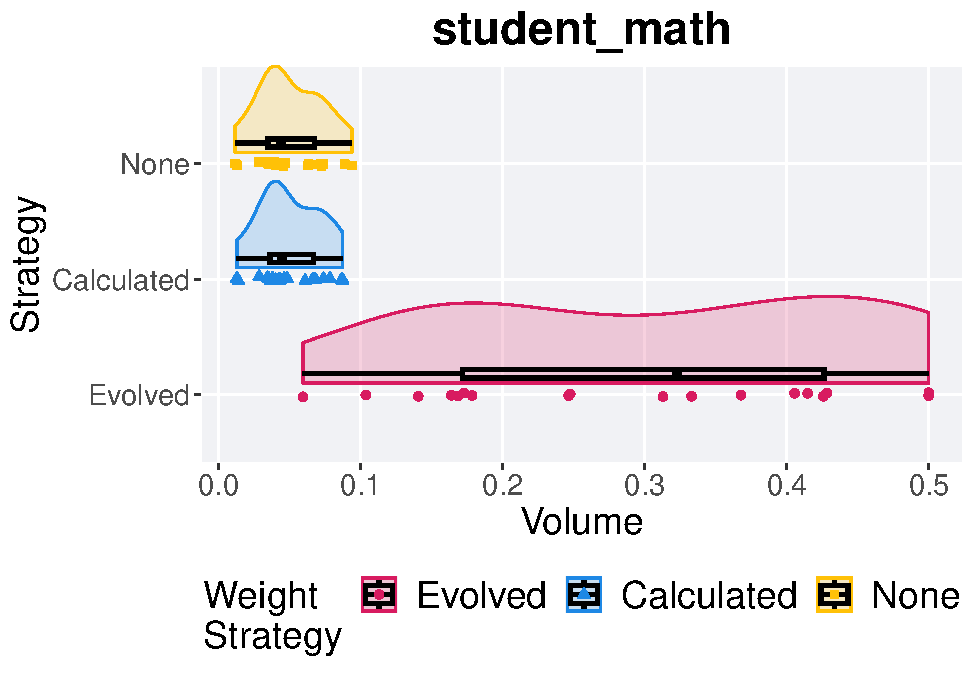
\includegraphics[width=1\linewidth]{evolved-sample-weights-supplemental_files/figure-latex/sm-hv-plt-1}

\hypertarget{summary-stats-1}{%
\subsection{Summary stats}\label{summary-stats-1}}

\begin{Shaded}
\begin{Highlighting}[]
\FunctionTok{volume\_summarize}\NormalTok{(data)}
\end{Highlighting}
\end{Shaded}

\begin{verbatim}
## # A tibble: 3 x 8
##   exp        count na_cnt    min median   mean    max    IQR
##   <fct>      <int>  <int>  <dbl>  <dbl>  <dbl>  <dbl>  <dbl>
## 1 Evolved       20      0 0.0594 0.323  0.308  0.5    0.255 
## 2 Calculated    20      0 0.0129 0.0448 0.0504 0.0873 0.0307
## 3 None          20      0 0.0116 0.0441 0.0503 0.0939 0.0326
\end{verbatim}

\hypertarget{kruskal-wallis-test-1}{%
\subsection{Kruskal-Wallis test}\label{kruskal-wallis-test-1}}

Detected differences between weight strategies.

\begin{Shaded}
\begin{Highlighting}[]
\FunctionTok{kruskal.test}\NormalTok{(hv }\SpecialCharTok{\textasciitilde{}}\NormalTok{ exp, }\AttributeTok{data =}\NormalTok{ data)}
\end{Highlighting}
\end{Shaded}

\begin{verbatim}
## 
##  Kruskal-Wallis rank sum test
## 
## data:  hv by exp
## Kruskal-Wallis chi-squared = 36.282, df = 2, p-value = 1.323e-08
\end{verbatim}

\hypertarget{pairwise-wlcoxon-test-1}{%
\subsection{Pairwise wlcoxon test}\label{pairwise-wlcoxon-test-1}}

\begin{Shaded}
\begin{Highlighting}[]
\FunctionTok{pairwise.wilcox.test}\NormalTok{(}\AttributeTok{x =}\NormalTok{ data}\SpecialCharTok{$}\NormalTok{hv, }\AttributeTok{g =}\NormalTok{ data}\SpecialCharTok{$}\NormalTok{exp, }\AttributeTok{p.adjust.method =} \StringTok{"bonferroni"}\NormalTok{,}
                    \AttributeTok{paired =} \ConstantTok{FALSE}\NormalTok{, }\AttributeTok{conf.int =} \ConstantTok{FALSE}\NormalTok{, }\AttributeTok{alternative =} \StringTok{\textquotesingle{}l\textquotesingle{}}\NormalTok{)}
\end{Highlighting}
\end{Shaded}

\begin{verbatim}
## 
##  Pairwise comparisons using Wilcoxon rank sum test with continuity correction 
## 
## data:  data$hv and data$exp 
## 
##            Evolved Calculated
## Calculated 3.3e-07 -         
## None       3.3e-07 1         
## 
## P value adjustment method: bonferroni
\end{verbatim}

\hypertarget{student-por}{%
\chapter{Student Por}\label{student-por}}

Here we report the \textbf{hypervolume} achived by evaluating the performance of each solution wihtin the Pareto front on the test set of the \texttt{student\_por} dataset.

\begin{Shaded}
\begin{Highlighting}[]
\CommentTok{\# heart{-}disease data}
\NormalTok{data }\OtherTok{\textless{}{-}} \FunctionTok{filter}\NormalTok{(testing, dataset }\SpecialCharTok{==} \StringTok{"student\_por"}\NormalTok{)}
\end{Highlighting}
\end{Shaded}

\hypertarget{hypervolume-2}{%
\section{Hypervolume}\label{hypervolume-2}}

\begin{Shaded}
\begin{Highlighting}[]
\FunctionTok{volume\_plotter}\NormalTok{(data,}\DecValTok{3}\NormalTok{)}
\end{Highlighting}
\end{Shaded}

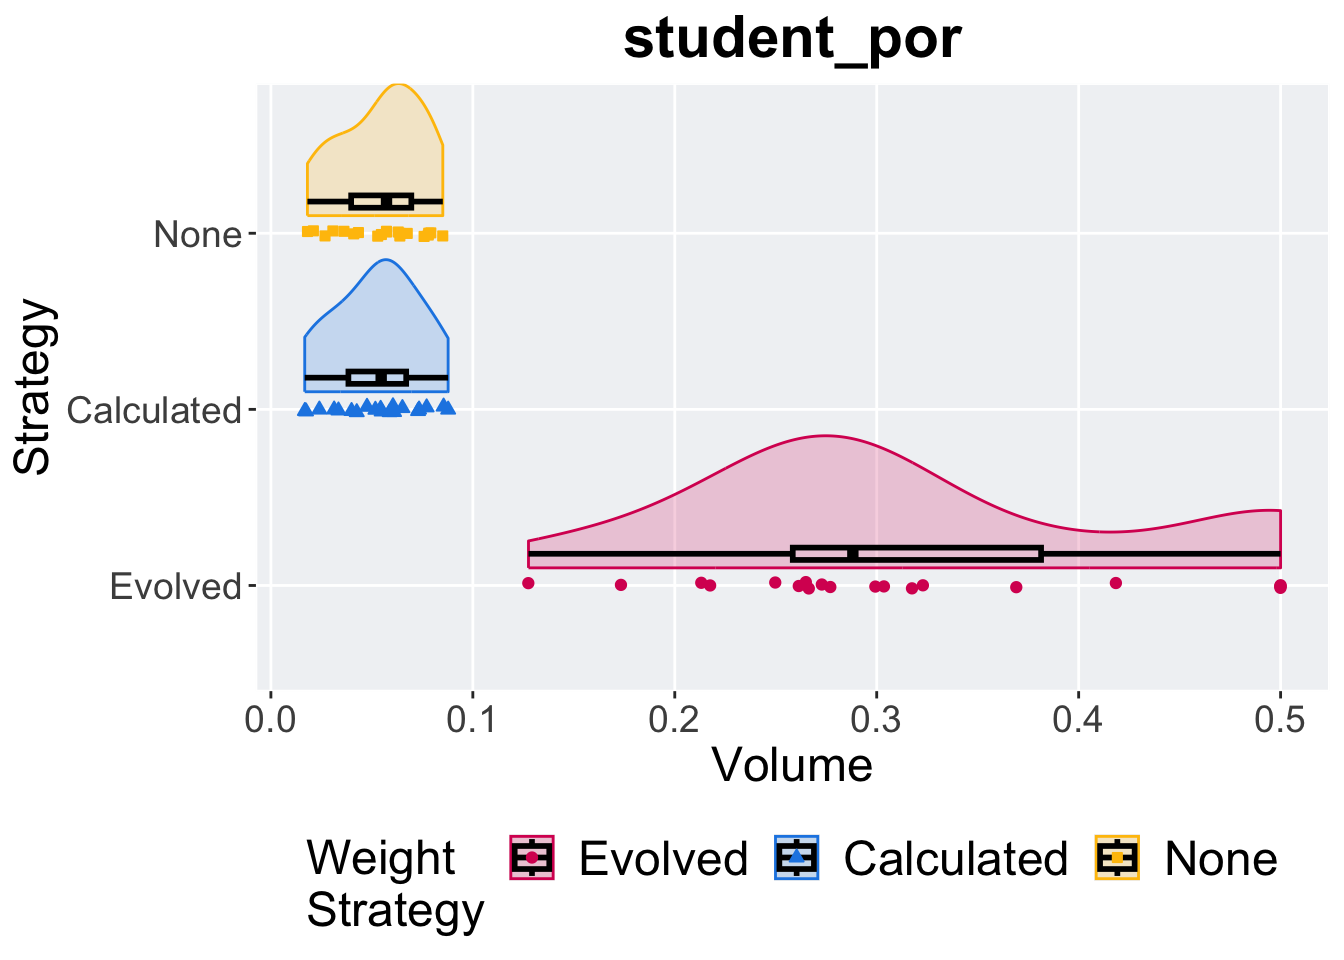
\includegraphics[width=1\linewidth]{evolved-sample-weights-supplemental_files/figure-latex/sp-hv-plt-1}

\hypertarget{summary-stats-2}{%
\subsection{Summary stats}\label{summary-stats-2}}

\begin{Shaded}
\begin{Highlighting}[]
\FunctionTok{volume\_summarize}\NormalTok{(data)}
\end{Highlighting}
\end{Shaded}

\begin{verbatim}
## # A tibble: 3 x 8
##   exp        count na_cnt    min median   mean    max    IQR
##   <fct>      <int>  <int>  <dbl>  <dbl>  <dbl>  <dbl>  <dbl>
## 1 Evolved       20      0 0.128  0.288  0.318  0.5    0.123 
## 2 Calculated    20      0 0.0168 0.0546 0.0528 0.0878 0.0286
## 3 None          20      0 0.0181 0.0573 0.0547 0.0851 0.0298
\end{verbatim}

\hypertarget{kruskal-wallis-test-2}{%
\subsection{Kruskal-Wallis test}\label{kruskal-wallis-test-2}}

Detected differences between weight strategies.

\begin{Shaded}
\begin{Highlighting}[]
\FunctionTok{kruskal.test}\NormalTok{(hv }\SpecialCharTok{\textasciitilde{}}\NormalTok{ exp, }\AttributeTok{data =}\NormalTok{ data)}
\end{Highlighting}
\end{Shaded}

\begin{verbatim}
## 
##  Kruskal-Wallis rank sum test
## 
## data:  hv by exp
## Kruskal-Wallis chi-squared = 39.429, df = 2, p-value = 2.742e-09
\end{verbatim}

\hypertarget{pairwise-wlcoxon-test-2}{%
\subsection{Pairwise wlcoxon test}\label{pairwise-wlcoxon-test-2}}

\begin{Shaded}
\begin{Highlighting}[]
\FunctionTok{pairwise.wilcox.test}\NormalTok{(}\AttributeTok{x =}\NormalTok{ data}\SpecialCharTok{$}\NormalTok{hv, }\AttributeTok{g =}\NormalTok{ data}\SpecialCharTok{$}\NormalTok{exp, }\AttributeTok{p.adjust.method =} \StringTok{"bonferroni"}\NormalTok{,}
                    \AttributeTok{paired =} \ConstantTok{FALSE}\NormalTok{, }\AttributeTok{conf.int =} \ConstantTok{FALSE}\NormalTok{, }\AttributeTok{alternative =} \StringTok{\textquotesingle{}l\textquotesingle{}}\NormalTok{)}
\end{Highlighting}
\end{Shaded}

\begin{verbatim}
## 
##  Pairwise comparisons using Wilcoxon rank sum test with continuity correction 
## 
## data:  data$hv and data$exp 
## 
##            Evolved Calculated
## Calculated 1e-07   -         
## None       1e-07   1         
## 
## P value adjustment method: bonferroni
\end{verbatim}

\hypertarget{creditg}{%
\chapter{CreditG}\label{creditg}}

Here we report the \textbf{hypervolume} achived by evaluating the performance of each solution wihtin the Pareto front on the test set of the \texttt{creditg} dataset.

\begin{Shaded}
\begin{Highlighting}[]
\CommentTok{\# heart{-}disease data}
\NormalTok{data }\OtherTok{\textless{}{-}} \FunctionTok{filter}\NormalTok{(testing, dataset }\SpecialCharTok{==} \StringTok{"creditg"}\NormalTok{)}
\end{Highlighting}
\end{Shaded}

\hypertarget{hypervolume-3}{%
\section{Hypervolume}\label{hypervolume-3}}

\begin{Shaded}
\begin{Highlighting}[]
\FunctionTok{volume\_plotter}\NormalTok{(data,}\DecValTok{4}\NormalTok{)}
\end{Highlighting}
\end{Shaded}

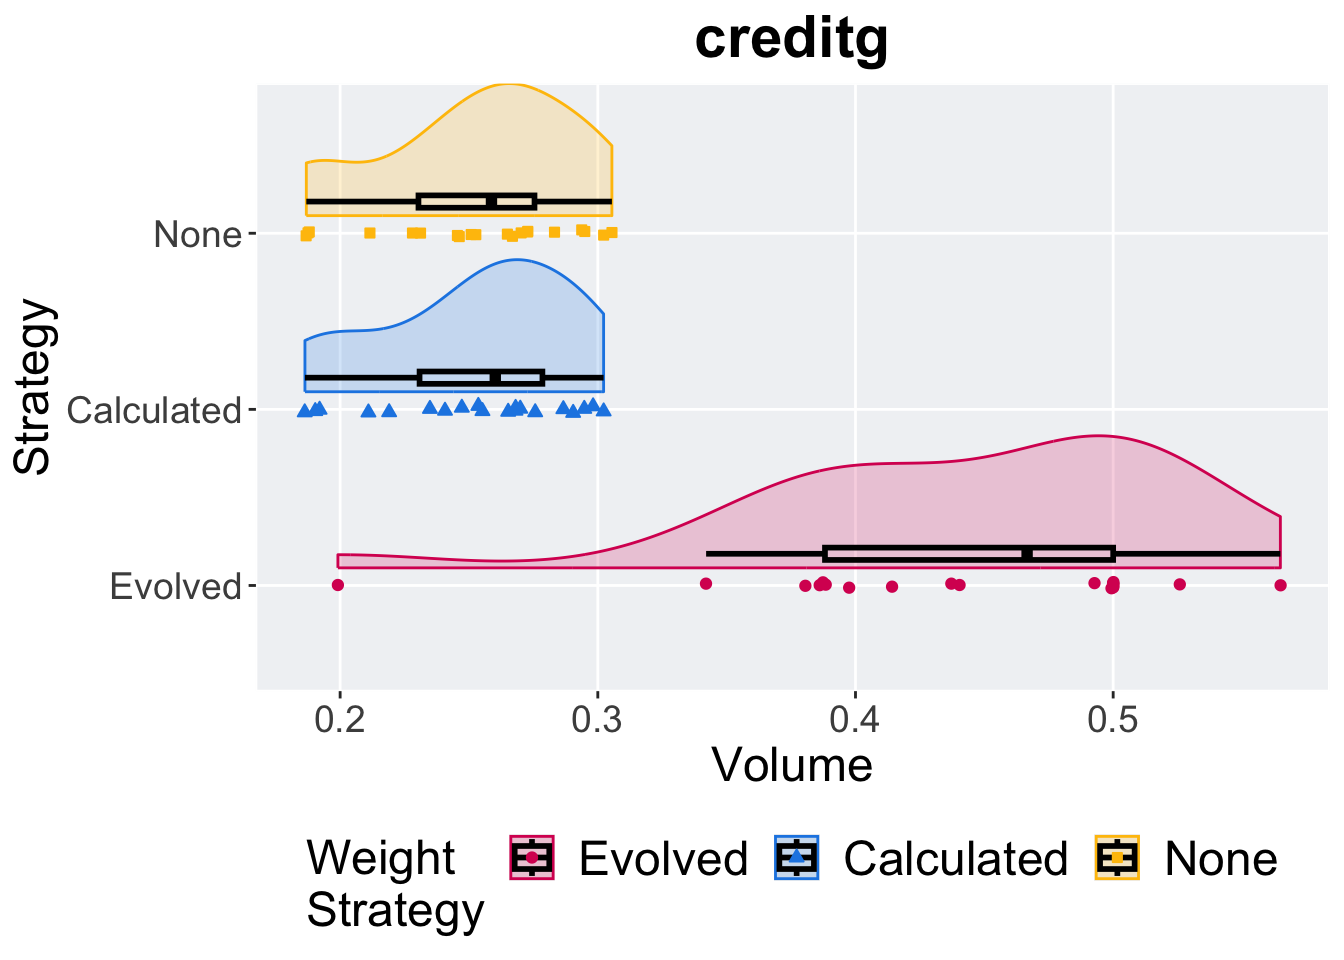
\includegraphics[width=1\linewidth]{evolved-sample-weights-supplemental_files/figure-latex/cg-hv-plt-1}

\hypertarget{summary-stats-3}{%
\subsection{Summary stats}\label{summary-stats-3}}

\begin{Shaded}
\begin{Highlighting}[]
\FunctionTok{volume\_summarize}\NormalTok{(data)}
\end{Highlighting}
\end{Shaded}

\begin{verbatim}
## # A tibble: 3 x 8
##   exp        count na_cnt   min median  mean   max    IQR
##   <fct>      <int>  <int> <dbl>  <dbl> <dbl> <dbl>  <dbl>
## 1 Evolved       20      0 0.199  0.467 0.443 0.565 0.112 
## 2 Calculated    20      0 0.186  0.260 0.252 0.302 0.0477
## 3 None          20      0 0.187  0.259 0.253 0.305 0.0450
\end{verbatim}

\hypertarget{kruskal-wallis-test-3}{%
\subsection{Kruskal-Wallis test}\label{kruskal-wallis-test-3}}

Detected differences between weight strategies.

\begin{Shaded}
\begin{Highlighting}[]
\FunctionTok{kruskal.test}\NormalTok{(hv }\SpecialCharTok{\textasciitilde{}}\NormalTok{ exp, }\AttributeTok{data =}\NormalTok{ data)}
\end{Highlighting}
\end{Shaded}

\begin{verbatim}
## 
##  Kruskal-Wallis rank sum test
## 
## data:  hv by exp
## Kruskal-Wallis chi-squared = 32.972, df = 2, p-value = 6.922e-08
\end{verbatim}

\hypertarget{pairwise-wlcoxon-test-3}{%
\subsection{Pairwise wlcoxon test}\label{pairwise-wlcoxon-test-3}}

\begin{Shaded}
\begin{Highlighting}[]
\FunctionTok{pairwise.wilcox.test}\NormalTok{(}\AttributeTok{x =}\NormalTok{ data}\SpecialCharTok{$}\NormalTok{hv, }\AttributeTok{g =}\NormalTok{ data}\SpecialCharTok{$}\NormalTok{exp, }\AttributeTok{p.adjust.method =} \StringTok{"bonferroni"}\NormalTok{,}
                    \AttributeTok{paired =} \ConstantTok{FALSE}\NormalTok{, }\AttributeTok{conf.int =} \ConstantTok{FALSE}\NormalTok{, }\AttributeTok{alternative =} \StringTok{\textquotesingle{}l\textquotesingle{}}\NormalTok{)}
\end{Highlighting}
\end{Shaded}

\begin{verbatim}
## 
##  Pairwise comparisons using Wilcoxon rank sum test with continuity correction 
## 
## data:  data$hv and data$exp 
## 
##            Evolved Calculated
## Calculated 1.1e-06 -         
## None       1.1e-06 1         
## 
## P value adjustment method: bonferroni
\end{verbatim}

\hypertarget{titanic}{%
\chapter{Titanic}\label{titanic}}

Here we report the \textbf{hypervolume} achived by evaluating the performance of each solution wihtin the Pareto front on the test set of the \texttt{titanic} dataset.

\begin{Shaded}
\begin{Highlighting}[]
\CommentTok{\# heart{-}disease data}
\NormalTok{data }\OtherTok{\textless{}{-}} \FunctionTok{filter}\NormalTok{(testing, dataset }\SpecialCharTok{==} \StringTok{"titanic"}\NormalTok{)}
\end{Highlighting}
\end{Shaded}

\hypertarget{hypervolume-4}{%
\section{Hypervolume}\label{hypervolume-4}}

\begin{Shaded}
\begin{Highlighting}[]
\FunctionTok{volume\_plotter}\NormalTok{(data,}\DecValTok{5}\NormalTok{)}
\end{Highlighting}
\end{Shaded}

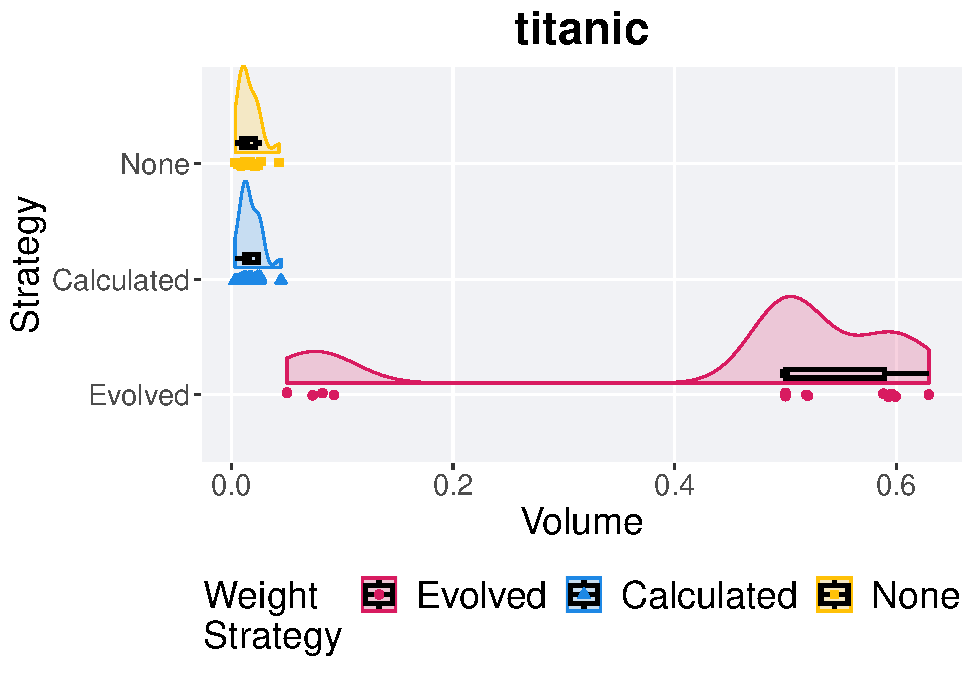
\includegraphics[width=1\linewidth]{evolved-sample-weights-supplemental_files/figure-latex/ti-hv-plt-1}

\hypertarget{summary-stats-4}{%
\subsection{Summary stats}\label{summary-stats-4}}

\begin{Shaded}
\begin{Highlighting}[]
\FunctionTok{volume\_summarize}\NormalTok{(data)}
\end{Highlighting}
\end{Shaded}

\begin{verbatim}
## # A tibble: 3 x 8
##   exp        count na_cnt     min median   mean    max    IQR
##   <fct>      <int>  <int>   <dbl>  <dbl>  <dbl>  <dbl>  <dbl>
## 1 Evolved       20      0 0.0502  0.5    0.447  0.629  0.0894
## 2 Calculated    20      0 0.00334 0.0143 0.0171 0.0448 0.0119
## 3 None          20      0 0.00340 0.0126 0.0157 0.0430 0.0125
\end{verbatim}

\hypertarget{kruskal-wallis-test-4}{%
\subsection{Kruskal-Wallis test}\label{kruskal-wallis-test-4}}

Detected differences between weight strategies.

\begin{Shaded}
\begin{Highlighting}[]
\FunctionTok{kruskal.test}\NormalTok{(hv }\SpecialCharTok{\textasciitilde{}}\NormalTok{ exp, }\AttributeTok{data =}\NormalTok{ data)}
\end{Highlighting}
\end{Shaded}

\begin{verbatim}
## 
##  Kruskal-Wallis rank sum test
## 
## data:  hv by exp
## Kruskal-Wallis chi-squared = 39.658, df = 2, p-value = 2.445e-09
\end{verbatim}

\hypertarget{pairwise-wlcoxon-test-4}{%
\subsection{Pairwise wlcoxon test}\label{pairwise-wlcoxon-test-4}}

\begin{Shaded}
\begin{Highlighting}[]
\FunctionTok{pairwise.wilcox.test}\NormalTok{(}\AttributeTok{x =}\NormalTok{ data}\SpecialCharTok{$}\NormalTok{hv, }\AttributeTok{g =}\NormalTok{ data}\SpecialCharTok{$}\NormalTok{exp, }\AttributeTok{p.adjust.method =} \StringTok{"bonferroni"}\NormalTok{,}
                    \AttributeTok{paired =} \ConstantTok{FALSE}\NormalTok{, }\AttributeTok{conf.int =} \ConstantTok{FALSE}\NormalTok{, }\AttributeTok{alternative =} \StringTok{\textquotesingle{}l\textquotesingle{}}\NormalTok{)}
\end{Highlighting}
\end{Shaded}

\begin{verbatim}
## 
##  Pairwise comparisons using Wilcoxon rank sum test with continuity correction 
## 
## data:  data$hv and data$exp 
## 
##            Evolved Calculated
## Calculated 9e-08   -         
## None       9e-08   0.74      
## 
## P value adjustment method: bonferroni
\end{verbatim}

\hypertarget{us-crime}{%
\chapter{US Crime}\label{us-crime}}

Here we report the \textbf{hypervolume} achived by evaluating the performance of each solution wihtin the Pareto front on the test set of the \texttt{us\_crime} dataset.

\begin{Shaded}
\begin{Highlighting}[]
\CommentTok{\# heart{-}disease data}
\NormalTok{data }\OtherTok{\textless{}{-}} \FunctionTok{filter}\NormalTok{(testing, dataset }\SpecialCharTok{==} \StringTok{"us\_crime"}\NormalTok{)}
\end{Highlighting}
\end{Shaded}

\hypertarget{hypervolume-5}{%
\section{Hypervolume}\label{hypervolume-5}}

\begin{Shaded}
\begin{Highlighting}[]
\FunctionTok{volume\_plotter}\NormalTok{(data,}\DecValTok{6}\NormalTok{)}
\end{Highlighting}
\end{Shaded}

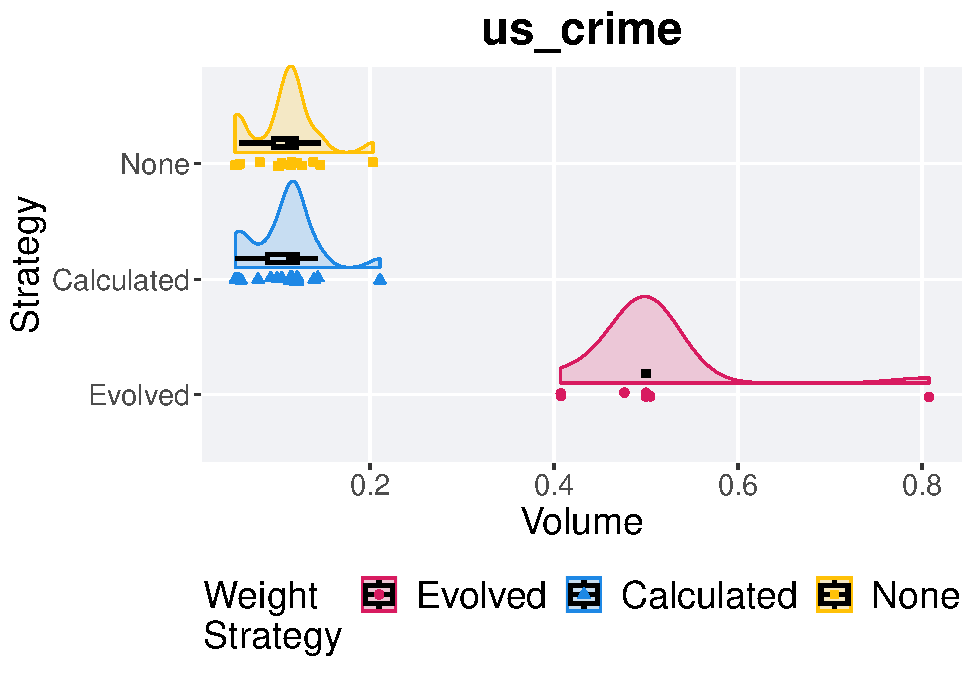
\includegraphics[width=1\linewidth]{evolved-sample-weights-supplemental_files/figure-latex/usc-hv-plt-1}

\hypertarget{summary-stats-5}{%
\subsection{Summary stats}\label{summary-stats-5}}

\begin{Shaded}
\begin{Highlighting}[]
\FunctionTok{volume\_summarize}\NormalTok{(data)}
\end{Highlighting}
\end{Shaded}

\begin{verbatim}
## # A tibble: 3 x 8
##   exp        count na_cnt    min median  mean   max    IQR
##   <fct>      <int>  <int>  <dbl>  <dbl> <dbl> <dbl>  <dbl>
## 1 Evolved       20      0 0.407   0.5   0.505 0.807 0     
## 2 Calculated    20      0 0.0536  0.114 0.108 0.211 0.0322
## 3 None          20      0 0.0534  0.113 0.107 0.203 0.0252
\end{verbatim}

\hypertarget{kruskal-wallis-test-5}{%
\subsection{Kruskal-Wallis test}\label{kruskal-wallis-test-5}}

Detected differences between weight strategies.

\begin{Shaded}
\begin{Highlighting}[]
\FunctionTok{kruskal.test}\NormalTok{(hv }\SpecialCharTok{\textasciitilde{}}\NormalTok{ exp, }\AttributeTok{data =}\NormalTok{ data)}
\end{Highlighting}
\end{Shaded}

\begin{verbatim}
## 
##  Kruskal-Wallis rank sum test
## 
## data:  hv by exp
## Kruskal-Wallis chi-squared = 39.978, df = 2, p-value = 2.084e-09
\end{verbatim}

\hypertarget{pairwise-wlcoxon-test-5}{%
\subsection{Pairwise wlcoxon test}\label{pairwise-wlcoxon-test-5}}

\begin{Shaded}
\begin{Highlighting}[]
\FunctionTok{pairwise.wilcox.test}\NormalTok{(}\AttributeTok{x =}\NormalTok{ data}\SpecialCharTok{$}\NormalTok{hv, }\AttributeTok{g =}\NormalTok{ data}\SpecialCharTok{$}\NormalTok{exp, }\AttributeTok{p.adjust.method =} \StringTok{"bonferroni"}\NormalTok{,}
                    \AttributeTok{paired =} \ConstantTok{FALSE}\NormalTok{, }\AttributeTok{conf.int =} \ConstantTok{FALSE}\NormalTok{, }\AttributeTok{alternative =} \StringTok{\textquotesingle{}l\textquotesingle{}}\NormalTok{)}
\end{Highlighting}
\end{Shaded}

\begin{verbatim}
## 
##  Pairwise comparisons using Wilcoxon rank sum test with continuity correction 
## 
## data:  data$hv and data$exp 
## 
##            Evolved Calculated
## Calculated 4.4e-08 -         
## None       4.4e-08 1         
## 
## P value adjustment method: bonferroni
\end{verbatim}

\hypertarget{compas-violent}{%
\chapter{Compas Violent}\label{compas-violent}}

Here we report the \textbf{hypervolume} achived by evaluating the performance of each solution wihtin the Pareto front on the test set of the \texttt{compas\_violent} dataset.

\begin{Shaded}
\begin{Highlighting}[]
\CommentTok{\# heart{-}disease data}
\NormalTok{data }\OtherTok{\textless{}{-}} \FunctionTok{filter}\NormalTok{(testing, dataset }\SpecialCharTok{==} \StringTok{"compas\_violent"}\NormalTok{)}
\end{Highlighting}
\end{Shaded}

\hypertarget{hypervolume-6}{%
\section{Hypervolume}\label{hypervolume-6}}

\begin{Shaded}
\begin{Highlighting}[]
\FunctionTok{volume\_plotter}\NormalTok{(data,}\DecValTok{7}\NormalTok{)}
\end{Highlighting}
\end{Shaded}

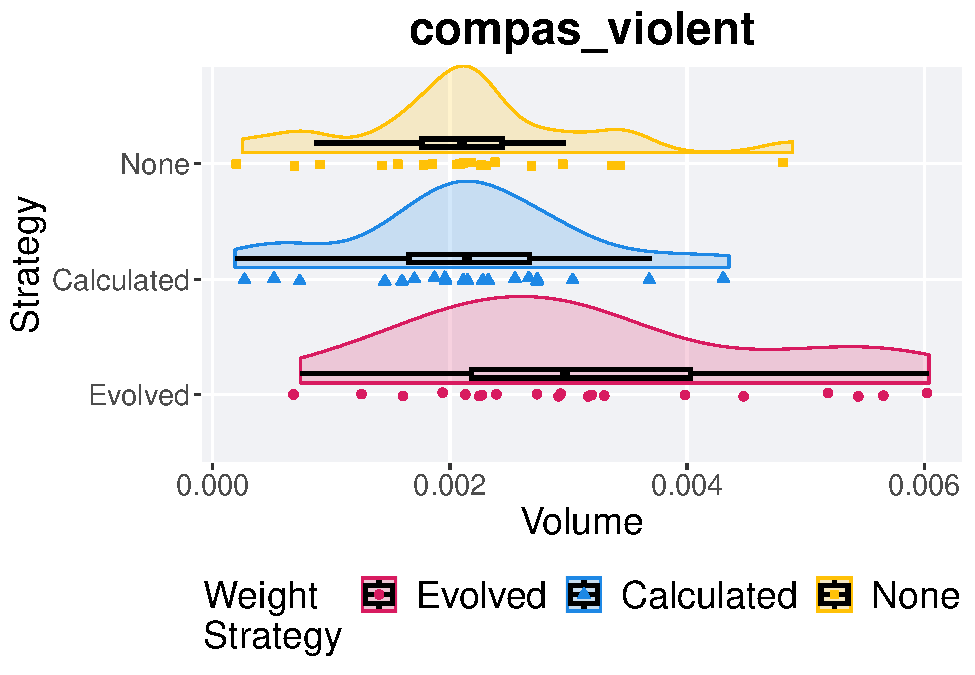
\includegraphics[width=1\linewidth]{evolved-sample-weights-supplemental_files/figure-latex/cv-hv-plt-1}

\hypertarget{summary-stats-6}{%
\subsection{Summary stats}\label{summary-stats-6}}

\begin{Shaded}
\begin{Highlighting}[]
\FunctionTok{volume\_summarize}\NormalTok{(data)}
\end{Highlighting}
\end{Shaded}

\begin{verbatim}
## # A tibble: 3 x 8
##   exp        count na_cnt      min  median    mean     max      IQR
##   <fct>      <int>  <int>    <dbl>   <dbl>   <dbl>   <dbl>    <dbl>
## 1 Evolved       20      0 0.000741 0.00297 0.00319 0.00604 0.00185 
## 2 Calculated    20      0 0.000188 0.00215 0.00215 0.00435 0.00101 
## 3 None          20      0 0.000251 0.00210 0.00217 0.00489 0.000675
\end{verbatim}

\hypertarget{kruskal-wallis-test-6}{%
\subsection{Kruskal-Wallis test}\label{kruskal-wallis-test-6}}

Detected differences between weight strategies.

\begin{Shaded}
\begin{Highlighting}[]
\FunctionTok{kruskal.test}\NormalTok{(hv }\SpecialCharTok{\textasciitilde{}}\NormalTok{ exp, }\AttributeTok{data =}\NormalTok{ data)}
\end{Highlighting}
\end{Shaded}

\begin{verbatim}
## 
##  Kruskal-Wallis rank sum test
## 
## data:  hv by exp
## Kruskal-Wallis chi-squared = 6.7764, df = 2, p-value = 0.03377
\end{verbatim}

\hypertarget{pairwise-wlcoxon-test-6}{%
\subsection{Pairwise wlcoxon test}\label{pairwise-wlcoxon-test-6}}

\begin{Shaded}
\begin{Highlighting}[]
\FunctionTok{pairwise.wilcox.test}\NormalTok{(}\AttributeTok{x =}\NormalTok{ data}\SpecialCharTok{$}\NormalTok{hv, }\AttributeTok{g =}\NormalTok{ data}\SpecialCharTok{$}\NormalTok{exp, }\AttributeTok{p.adjust.method =} \StringTok{"bonferroni"}\NormalTok{,}
                    \AttributeTok{paired =} \ConstantTok{FALSE}\NormalTok{, }\AttributeTok{conf.int =} \ConstantTok{FALSE}\NormalTok{, }\AttributeTok{alternative =} \StringTok{\textquotesingle{}l\textquotesingle{}}\NormalTok{)}
\end{Highlighting}
\end{Shaded}

\begin{verbatim}
## 
##  Pairwise comparisons using Wilcoxon rank sum exact test 
## 
## data:  data$hv and data$exp 
## 
##            Evolved Calculated
## Calculated 0.034   -         
## None       0.039   1.000     
## 
## P value adjustment method: bonferroni
\end{verbatim}

\hypertarget{nlsy}{%
\chapter{NLSY}\label{nlsy}}

Here we report the \textbf{hypervolume} achived by evaluating the performance of each solution wihtin the Pareto front on the test set of the \texttt{nlsy} dataset.

\begin{Shaded}
\begin{Highlighting}[]
\CommentTok{\# heart{-}disease data}
\NormalTok{data }\OtherTok{\textless{}{-}} \FunctionTok{filter}\NormalTok{(testing, dataset }\SpecialCharTok{==} \StringTok{"nlsy"}\NormalTok{)}
\end{Highlighting}
\end{Shaded}

\hypertarget{hypervolume-7}{%
\section{Hypervolume}\label{hypervolume-7}}

\begin{Shaded}
\begin{Highlighting}[]
\FunctionTok{volume\_plotter}\NormalTok{(data,}\DecValTok{8}\NormalTok{)}
\end{Highlighting}
\end{Shaded}

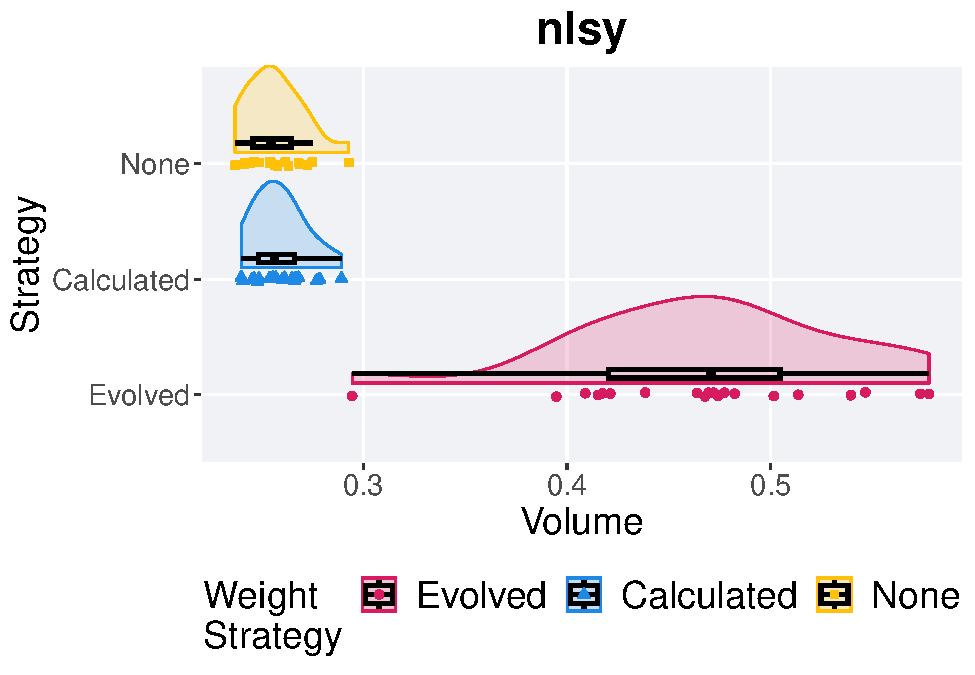
\includegraphics[width=1\linewidth]{evolved-sample-weights-supplemental_files/figure-latex/nsly-hv-plt-1}

\hypertarget{summary-stats-7}{%
\subsection{Summary stats}\label{summary-stats-7}}

\begin{Shaded}
\begin{Highlighting}[]
\FunctionTok{volume\_summarize}\NormalTok{(data)}
\end{Highlighting}
\end{Shaded}

\begin{verbatim}
## # A tibble: 3 x 8
##   exp        count na_cnt   min median  mean   max    IQR
##   <fct>      <int>  <int> <dbl>  <dbl> <dbl> <dbl>  <dbl>
## 1 Evolved       20      0 0.294  0.471 0.468 0.578 0.0843
## 2 Calculated    20      0 0.240  0.256 0.259 0.289 0.0177
## 3 None          20      0 0.237  0.254 0.256 0.293 0.0186
\end{verbatim}

\hypertarget{kruskal-wallis-test-7}{%
\subsection{Kruskal-Wallis test}\label{kruskal-wallis-test-7}}

Detected differences between weight strategies.

\begin{Shaded}
\begin{Highlighting}[]
\FunctionTok{kruskal.test}\NormalTok{(hv }\SpecialCharTok{\textasciitilde{}}\NormalTok{ exp, }\AttributeTok{data =}\NormalTok{ data)}
\end{Highlighting}
\end{Shaded}

\begin{verbatim}
## 
##  Kruskal-Wallis rank sum test
## 
## data:  hv by exp
## Kruskal-Wallis chi-squared = 39.518, df = 2, p-value = 2.623e-09
\end{verbatim}

\hypertarget{pairwise-wlcoxon-test-7}{%
\subsection{Pairwise wlcoxon test}\label{pairwise-wlcoxon-test-7}}

\begin{Shaded}
\begin{Highlighting}[]
\FunctionTok{pairwise.wilcox.test}\NormalTok{(}\AttributeTok{x =}\NormalTok{ data}\SpecialCharTok{$}\NormalTok{hv, }\AttributeTok{g =}\NormalTok{ data}\SpecialCharTok{$}\NormalTok{exp, }\AttributeTok{p.adjust.method =} \StringTok{"bonferroni"}\NormalTok{,}
                    \AttributeTok{paired =} \ConstantTok{FALSE}\NormalTok{, }\AttributeTok{conf.int =} \ConstantTok{FALSE}\NormalTok{, }\AttributeTok{alternative =} \StringTok{\textquotesingle{}l\textquotesingle{}}\NormalTok{)}
\end{Highlighting}
\end{Shaded}

\begin{verbatim}
## 
##  Pairwise comparisons using Wilcoxon rank sum exact test 
## 
## data:  data$hv and data$exp 
## 
##            Evolved Calculated
## Calculated 2.2e-11 -         
## None       2.2e-11 0.82      
## 
## P value adjustment method: bonferroni
\end{verbatim}

\hypertarget{compas}{%
\chapter{Compas}\label{compas}}

Here we report the \textbf{hypervolume} achived by evaluating the performance of each solution wihtin the Pareto front on the test set of the \texttt{compas} dataset.

\begin{Shaded}
\begin{Highlighting}[]
\CommentTok{\# heart{-}disease data}
\NormalTok{data }\OtherTok{\textless{}{-}} \FunctionTok{filter}\NormalTok{(testing, dataset }\SpecialCharTok{==} \StringTok{"compas"}\NormalTok{)}
\end{Highlighting}
\end{Shaded}

\hypertarget{hypervolume-8}{%
\section{Hypervolume}\label{hypervolume-8}}

\begin{Shaded}
\begin{Highlighting}[]
\FunctionTok{volume\_plotter}\NormalTok{(data,}\DecValTok{9}\NormalTok{)}
\end{Highlighting}
\end{Shaded}

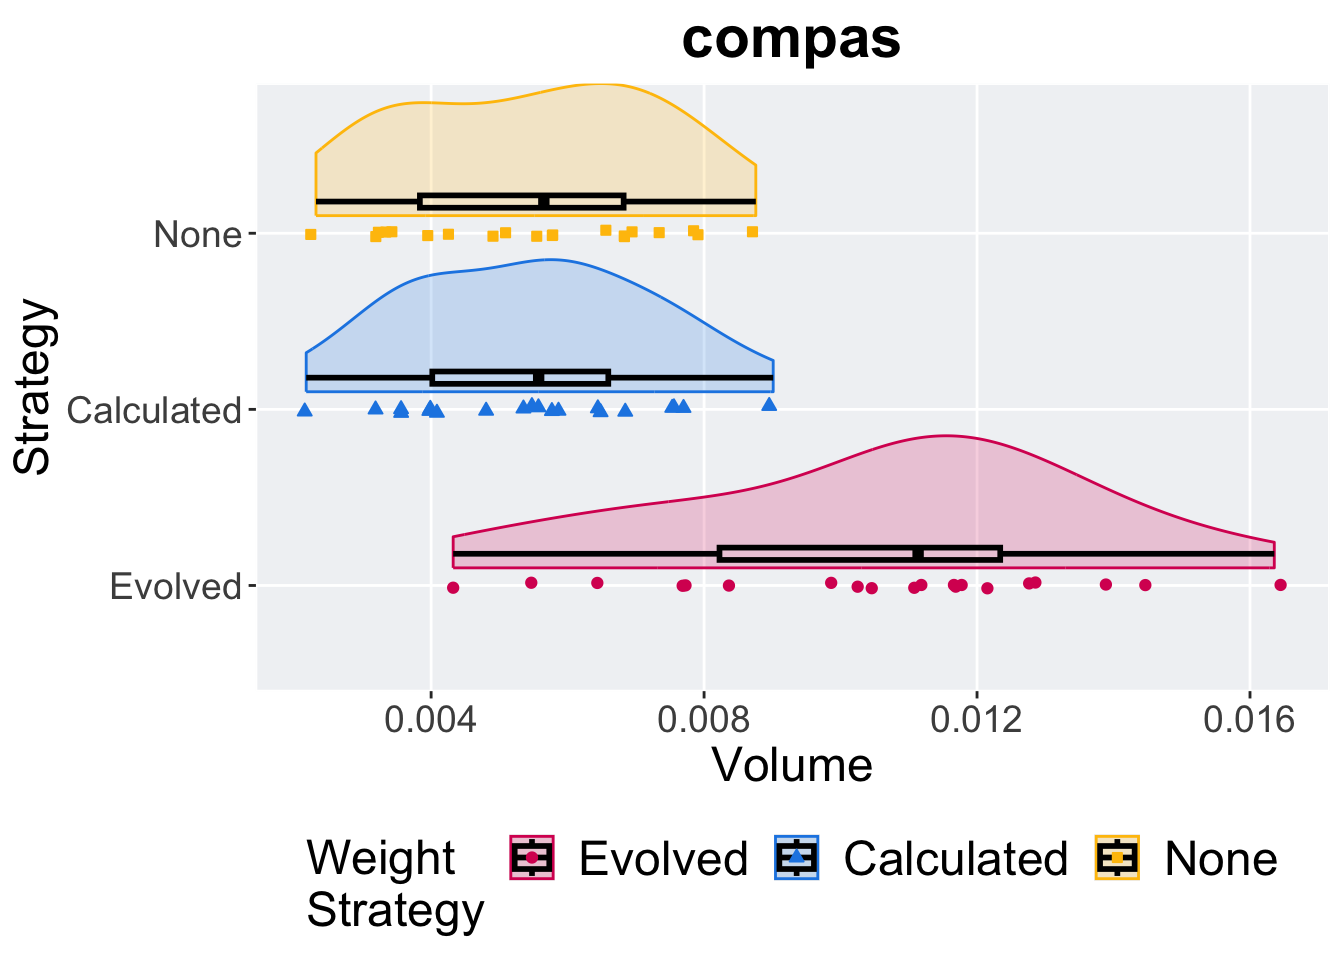
\includegraphics[width=1\linewidth]{evolved-sample-weights-supplemental_files/figure-latex/cp-hv-plt-1}

\hypertarget{summary-stats-8}{%
\subsection{Summary stats}\label{summary-stats-8}}

\begin{Shaded}
\begin{Highlighting}[]
\FunctionTok{volume\_summarize}\NormalTok{(data)}
\end{Highlighting}
\end{Shaded}

\begin{verbatim}
## # A tibble: 3 x 8
##   exp        count na_cnt     min  median    mean     max     IQR
##   <fct>      <int>  <int>   <dbl>   <dbl>   <dbl>   <dbl>   <dbl>
## 1 Evolved       20      0 0.00432 0.0111  0.0105  0.0164  0.00411
## 2 Calculated    20      0 0.00217 0.00558 0.00546 0.00901 0.00258
## 3 None          20      0 0.00231 0.00565 0.00548 0.00876 0.00299
\end{verbatim}

\hypertarget{kruskal-wallis-test-8}{%
\subsection{Kruskal-Wallis test}\label{kruskal-wallis-test-8}}

Detected differences between weight strategies.

\begin{Shaded}
\begin{Highlighting}[]
\FunctionTok{kruskal.test}\NormalTok{(hv }\SpecialCharTok{\textasciitilde{}}\NormalTok{ exp, }\AttributeTok{data =}\NormalTok{ data)}
\end{Highlighting}
\end{Shaded}

\begin{verbatim}
## 
##  Kruskal-Wallis rank sum test
## 
## data:  hv by exp
## Kruskal-Wallis chi-squared = 26.298, df = 2, p-value = 1.947e-06
\end{verbatim}

\hypertarget{pairwise-wlcoxon-test-8}{%
\subsection{Pairwise wlcoxon test}\label{pairwise-wlcoxon-test-8}}

\begin{Shaded}
\begin{Highlighting}[]
\FunctionTok{pairwise.wilcox.test}\NormalTok{(}\AttributeTok{x =}\NormalTok{ data}\SpecialCharTok{$}\NormalTok{hv, }\AttributeTok{g =}\NormalTok{ data}\SpecialCharTok{$}\NormalTok{exp, }\AttributeTok{p.adjust.method =} \StringTok{"bonferroni"}\NormalTok{,}
                    \AttributeTok{paired =} \ConstantTok{FALSE}\NormalTok{, }\AttributeTok{conf.int =} \ConstantTok{FALSE}\NormalTok{, }\AttributeTok{alternative =} \StringTok{\textquotesingle{}l\textquotesingle{}}\NormalTok{)}
\end{Highlighting}
\end{Shaded}

\begin{verbatim}
## 
##  Pairwise comparisons using Wilcoxon rank sum exact test 
## 
## data:  data$hv and data$exp 
## 
##            Evolved Calculated
## Calculated 1.4e-06 -         
## None       3.6e-06 1         
## 
## P value adjustment method: bonferroni
\end{verbatim}

\hypertarget{speeddating}{%
\chapter{Speeddating}\label{speeddating}}

Here we report the \textbf{hypervolume} achived by evaluating the performance of each solution wihtin the Pareto front on the test set of the \texttt{speeddating} dataset.

\begin{Shaded}
\begin{Highlighting}[]
\CommentTok{\# heart{-}disease data}
\NormalTok{data }\OtherTok{\textless{}{-}} \FunctionTok{filter}\NormalTok{(testing, dataset }\SpecialCharTok{==} \StringTok{"speeddating"}\NormalTok{)}
\end{Highlighting}
\end{Shaded}

\hypertarget{hypervolume-9}{%
\section{Hypervolume}\label{hypervolume-9}}

\begin{Shaded}
\begin{Highlighting}[]
\FunctionTok{volume\_plotter}\NormalTok{(data,}\DecValTok{10}\NormalTok{)}
\end{Highlighting}
\end{Shaded}

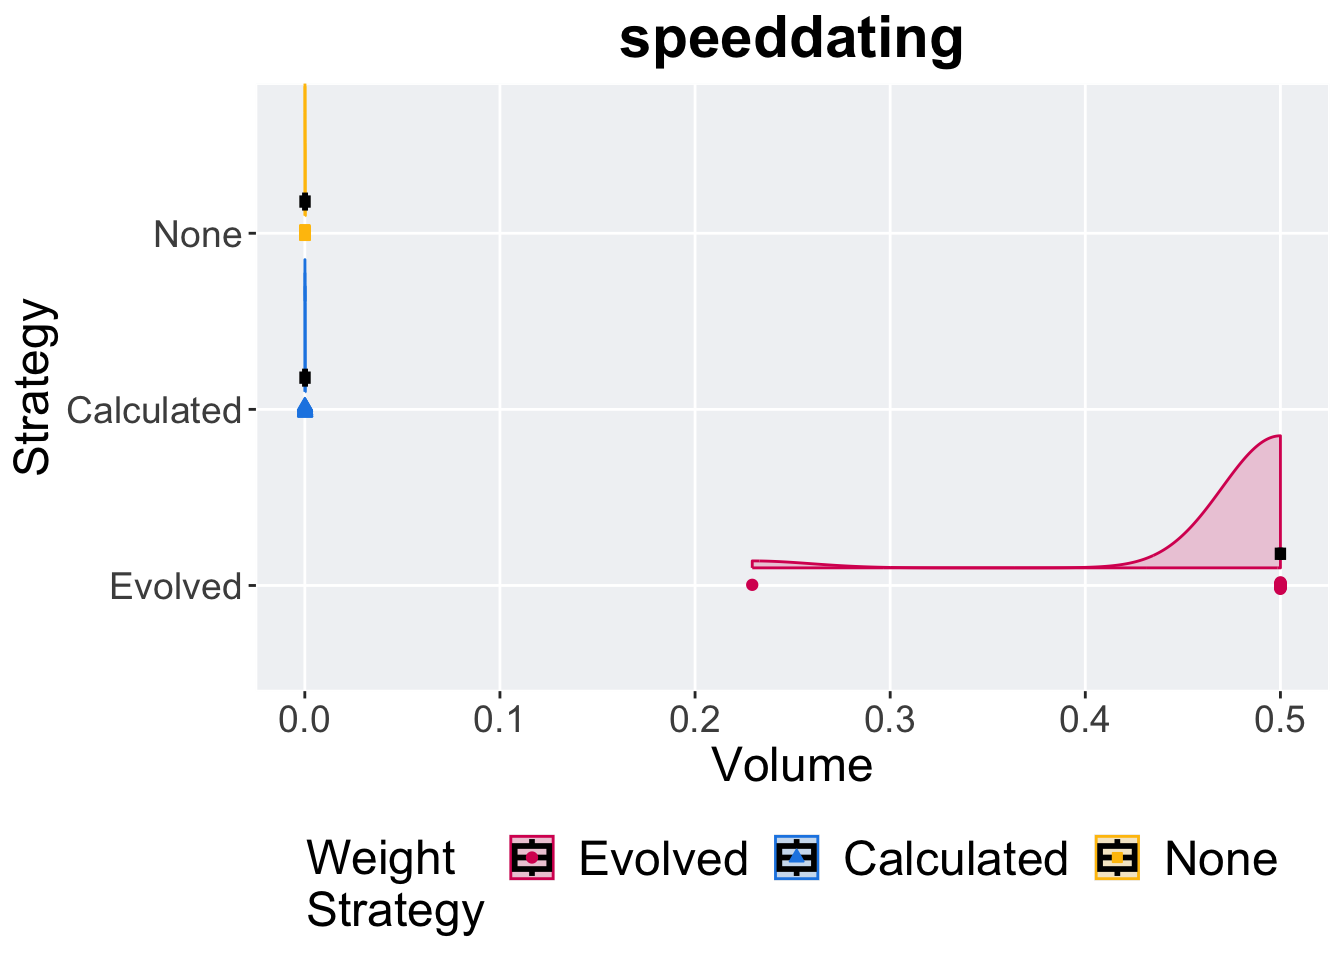
\includegraphics[width=1\linewidth]{evolved-sample-weights-supplemental_files/figure-latex/sd-hv-plt-1}

\hypertarget{summary-stats-9}{%
\subsection{Summary stats}\label{summary-stats-9}}

\begin{Shaded}
\begin{Highlighting}[]
\FunctionTok{volume\_summarize}\NormalTok{(data)}
\end{Highlighting}
\end{Shaded}

\begin{verbatim}
## # A tibble: 3 x 8
##   exp        count na_cnt       min   median     mean      max      IQR
##   <fct>      <int>  <int>     <dbl>    <dbl>    <dbl>    <dbl>    <dbl>
## 1 Evolved       20      0 0.229     0.5      0.486    0.5      0       
## 2 Calculated    20      0 0.0000388 0.000102 0.000114 0.000239 0.000121
## 3 None          20      0 0.0000297 0.000109 0.000124 0.000255 0.000122
\end{verbatim}

\hypertarget{kruskal-wallis-test-9}{%
\subsection{Kruskal-Wallis test}\label{kruskal-wallis-test-9}}

Detected differences between weight strategies.

\begin{Shaded}
\begin{Highlighting}[]
\FunctionTok{kruskal.test}\NormalTok{(hv }\SpecialCharTok{\textasciitilde{}}\NormalTok{ exp, }\AttributeTok{data =}\NormalTok{ data)}
\end{Highlighting}
\end{Shaded}

\begin{verbatim}
## 
##  Kruskal-Wallis rank sum test
## 
## data:  hv by exp
## Kruskal-Wallis chi-squared = 40.672, df = 2, p-value = 1.473e-09
\end{verbatim}

\hypertarget{pairwise-wlcoxon-test-9}{%
\subsection{Pairwise wlcoxon test}\label{pairwise-wlcoxon-test-9}}

\begin{Shaded}
\begin{Highlighting}[]
\FunctionTok{pairwise.wilcox.test}\NormalTok{(}\AttributeTok{x =}\NormalTok{ data}\SpecialCharTok{$}\NormalTok{hv, }\AttributeTok{g =}\NormalTok{ data}\SpecialCharTok{$}\NormalTok{exp, }\AttributeTok{p.adjust.method =} \StringTok{"bonferroni"}\NormalTok{,}
                    \AttributeTok{paired =} \ConstantTok{FALSE}\NormalTok{, }\AttributeTok{conf.int =} \ConstantTok{FALSE}\NormalTok{, }\AttributeTok{alternative =} \StringTok{\textquotesingle{}l\textquotesingle{}}\NormalTok{)}
\end{Highlighting}
\end{Shaded}

\begin{verbatim}
## 
##  Pairwise comparisons using Wilcoxon rank sum test with continuity correction 
## 
## data:  data$hv and data$exp 
## 
##            Evolved Calculated
## Calculated 1.7e-08 -         
## None       1.7e-08 1         
## 
## P value adjustment method: bonferroni
\end{verbatim}

\hypertarget{pmad-epds}{%
\chapter{PMAD EPDS}\label{pmad-epds}}

Here we report the \textbf{hypervolume} achived by evaluating the performance of each solution wihtin the Pareto front on the test set of the \texttt{pmad\_epds} dataset.

\begin{Shaded}
\begin{Highlighting}[]
\CommentTok{\# heart{-}disease data}
\NormalTok{data }\OtherTok{\textless{}{-}} \FunctionTok{filter}\NormalTok{(testing, dataset }\SpecialCharTok{==} \StringTok{"pmad\_epds"}\NormalTok{)}
\end{Highlighting}
\end{Shaded}

\hypertarget{hypervolume-10}{%
\section{Hypervolume}\label{hypervolume-10}}

\begin{Shaded}
\begin{Highlighting}[]
\FunctionTok{volume\_plotter}\NormalTok{(data,}\DecValTok{11}\NormalTok{)}
\end{Highlighting}
\end{Shaded}

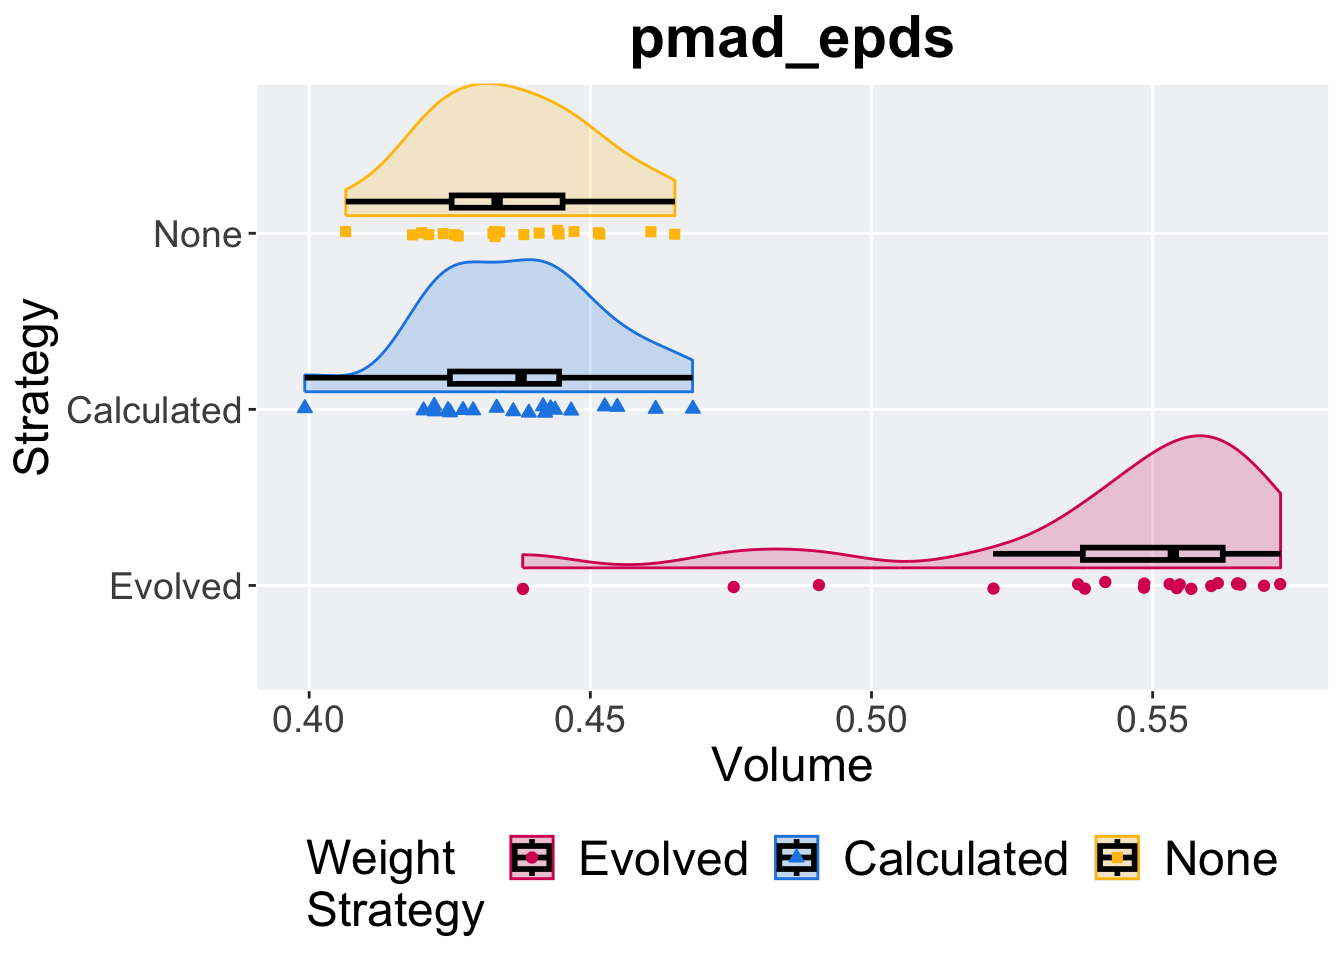
\includegraphics[width=1\linewidth]{evolved-sample-weights-supplemental_files/figure-latex/pe-hv-plt-1}

\hypertarget{summary-stats-10}{%
\subsection{Summary stats}\label{summary-stats-10}}

\begin{Shaded}
\begin{Highlighting}[]
\FunctionTok{volume\_summarize}\NormalTok{(data)}
\end{Highlighting}
\end{Shaded}

\begin{verbatim}
## # A tibble: 3 x 8
##   exp        count na_cnt   min median  mean   max    IQR
##   <fct>      <int>  <int> <dbl>  <dbl> <dbl> <dbl>  <dbl>
## 1 Evolved       20      0 0.438  0.554 0.541 0.573 0.0249
## 2 Calculated    20      0 0.399  0.438 0.437 0.468 0.0194
## 3 None          20      0 0.407  0.433 0.436 0.465 0.0197
\end{verbatim}

\hypertarget{kruskal-wallis-test-10}{%
\subsection{Kruskal-Wallis test}\label{kruskal-wallis-test-10}}

Detected differences between weight strategies.

\begin{Shaded}
\begin{Highlighting}[]
\FunctionTok{kruskal.test}\NormalTok{(hv }\SpecialCharTok{\textasciitilde{}}\NormalTok{ exp, }\AttributeTok{data =}\NormalTok{ data)}
\end{Highlighting}
\end{Shaded}

\begin{verbatim}
## 
##  Kruskal-Wallis rank sum test
## 
## data:  hv by exp
## Kruskal-Wallis chi-squared = 35.731, df = 2, p-value = 1.742e-08
\end{verbatim}

\hypertarget{pairwise-wlcoxon-test-10}{%
\subsection{Pairwise wlcoxon test}\label{pairwise-wlcoxon-test-10}}

\begin{Shaded}
\begin{Highlighting}[]
\FunctionTok{pairwise.wilcox.test}\NormalTok{(}\AttributeTok{x =}\NormalTok{ data}\SpecialCharTok{$}\NormalTok{hv, }\AttributeTok{g =}\NormalTok{ data}\SpecialCharTok{$}\NormalTok{exp, }\AttributeTok{p.adjust.method =} \StringTok{"bonferroni"}\NormalTok{,}
                    \AttributeTok{paired =} \ConstantTok{FALSE}\NormalTok{, }\AttributeTok{conf.int =} \ConstantTok{FALSE}\NormalTok{, }\AttributeTok{alternative =} \StringTok{\textquotesingle{}l\textquotesingle{}}\NormalTok{)}
\end{Highlighting}
\end{Shaded}

\begin{verbatim}
## 
##  Pairwise comparisons using Wilcoxon rank sum exact test 
## 
## data:  data$hv and data$exp 
## 
##            Evolved Calculated
## Calculated 3.0e-09 -         
## None       2.1e-09 1         
## 
## P value adjustment method: bonferroni
\end{verbatim}

\hypertarget{pmad-phq}{%
\chapter{PMAD PHQ}\label{pmad-phq}}

Here we report the \textbf{hypervolume} achived by evaluating the performance of each solution wihtin the Pareto front on the test set of the \texttt{pmad\_phq} dataset.

\begin{Shaded}
\begin{Highlighting}[]
\CommentTok{\# heart{-}disease data}
\NormalTok{data }\OtherTok{\textless{}{-}} \FunctionTok{filter}\NormalTok{(testing, dataset }\SpecialCharTok{==} \StringTok{"pmad\_phq"}\NormalTok{)}
\end{Highlighting}
\end{Shaded}

\hypertarget{hypervolume-11}{%
\section{Hypervolume}\label{hypervolume-11}}

\begin{Shaded}
\begin{Highlighting}[]
\FunctionTok{volume\_plotter}\NormalTok{(data,}\DecValTok{13}\NormalTok{)}
\end{Highlighting}
\end{Shaded}

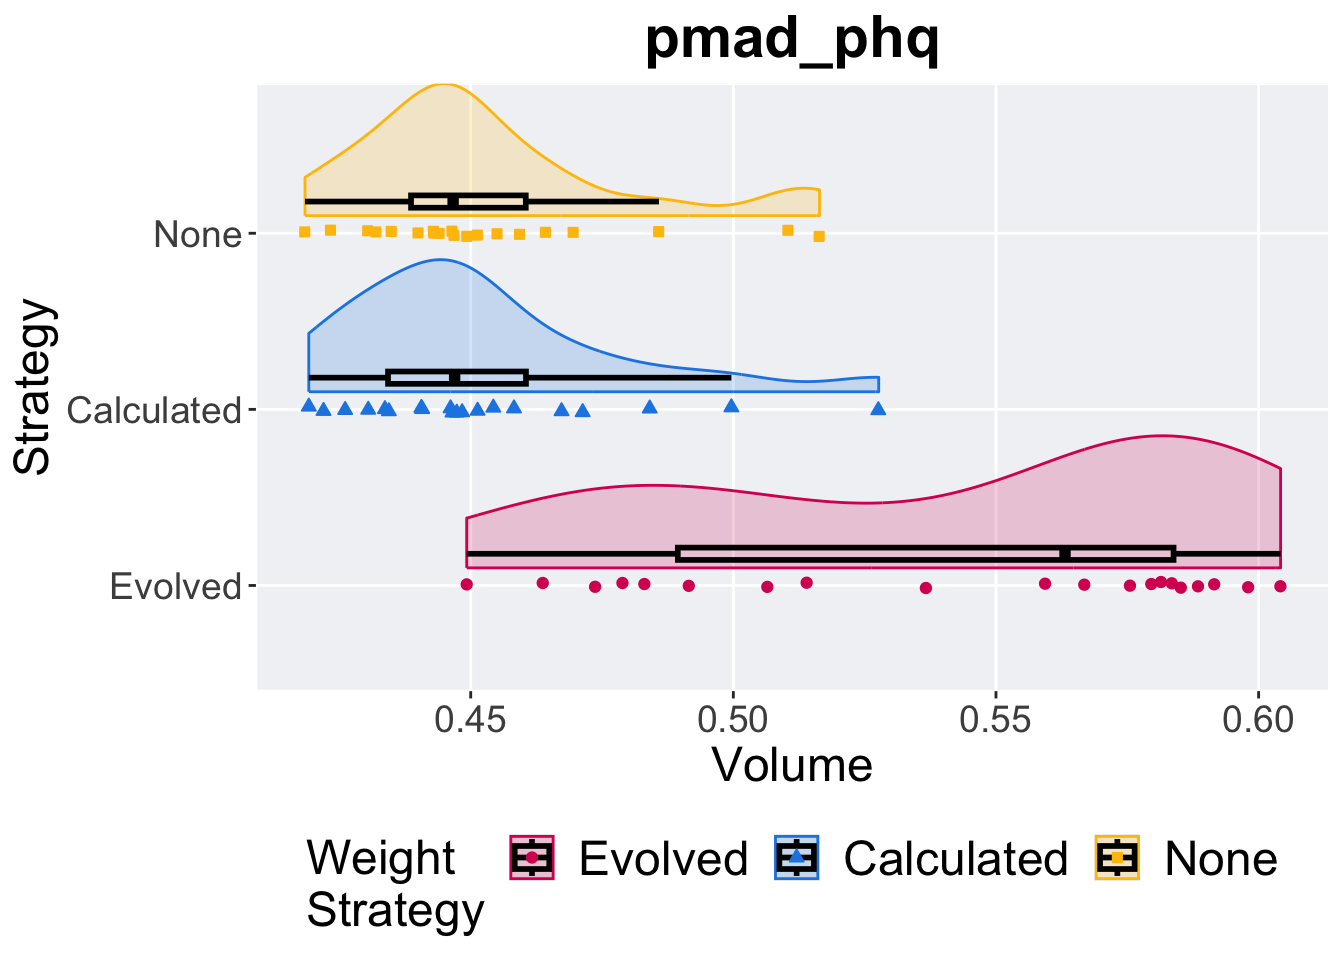
\includegraphics[width=1\linewidth]{evolved-sample-weights-supplemental_files/figure-latex/pp-hv-plt-1}

\hypertarget{summary-stats-11}{%
\subsection{Summary stats}\label{summary-stats-11}}

\begin{Shaded}
\begin{Highlighting}[]
\FunctionTok{volume\_summarize}\NormalTok{(data)}
\end{Highlighting}
\end{Shaded}

\begin{verbatim}
## # A tibble: 3 x 8
##   exp        count na_cnt   min median  mean   max    IQR
##   <fct>      <int>  <int> <dbl>  <dbl> <dbl> <dbl>  <dbl>
## 1 Evolved       20      0 0.449  0.563 0.541 0.604 0.0944
## 2 Calculated    20      0 0.419  0.447 0.452 0.528 0.0263
## 3 None          20      0 0.418  0.447 0.453 0.516 0.0218
\end{verbatim}

\hypertarget{kruskal-wallis-test-11}{%
\subsection{Kruskal-Wallis test}\label{kruskal-wallis-test-11}}

Detected differences between weight strategies.

\begin{Shaded}
\begin{Highlighting}[]
\FunctionTok{kruskal.test}\NormalTok{(hv }\SpecialCharTok{\textasciitilde{}}\NormalTok{ exp, }\AttributeTok{data =}\NormalTok{ data)}
\end{Highlighting}
\end{Shaded}

\begin{verbatim}
## 
##  Kruskal-Wallis rank sum test
## 
## data:  hv by exp
## Kruskal-Wallis chi-squared = 29.615, df = 2, p-value = 3.708e-07
\end{verbatim}

\hypertarget{pairwise-wlcoxon-test-11}{%
\subsection{Pairwise wlcoxon test}\label{pairwise-wlcoxon-test-11}}

\begin{Shaded}
\begin{Highlighting}[]
\FunctionTok{pairwise.wilcox.test}\NormalTok{(}\AttributeTok{x =}\NormalTok{ data}\SpecialCharTok{$}\NormalTok{hv, }\AttributeTok{g =}\NormalTok{ data}\SpecialCharTok{$}\NormalTok{exp, }\AttributeTok{p.adjust.method =} \StringTok{"bonferroni"}\NormalTok{,}
                    \AttributeTok{paired =} \ConstantTok{FALSE}\NormalTok{, }\AttributeTok{conf.int =} \ConstantTok{FALSE}\NormalTok{, }\AttributeTok{alternative =} \StringTok{\textquotesingle{}l\textquotesingle{}}\NormalTok{)}
\end{Highlighting}
\end{Shaded}

\begin{verbatim}
## 
##  Pairwise comparisons using Wilcoxon rank sum exact test 
## 
## data:  data$hv and data$exp 
## 
##            Evolved Calculated
## Calculated 2.5e-07 -         
## None       3.2e-07 1         
## 
## P value adjustment method: bonferroni
\end{verbatim}

  \bibliography{packages.bib,supplemental.bib}

\end{document}
